% gr-HoffmanSingleton.tex -- the Hoffman-Singleton graph : 50 vertices,
% 175 edges, 7-regular, girth 5 (a Moore graph).
% Robertson's construction : 5 pentagons P_h (P_hj ~ P_h(j+1)), 5
% pentagrams Q_i (Q_ij ~ Q_i(j+2)) and P_hj ~ Q_ik when k = hi+j mod 5.
% Engine : pdfLaTeX or LuaLaTeX
\documentclass[border=3mm, convert=false]{standalone}
\usepackage{tkz-berge}
\begin{document}
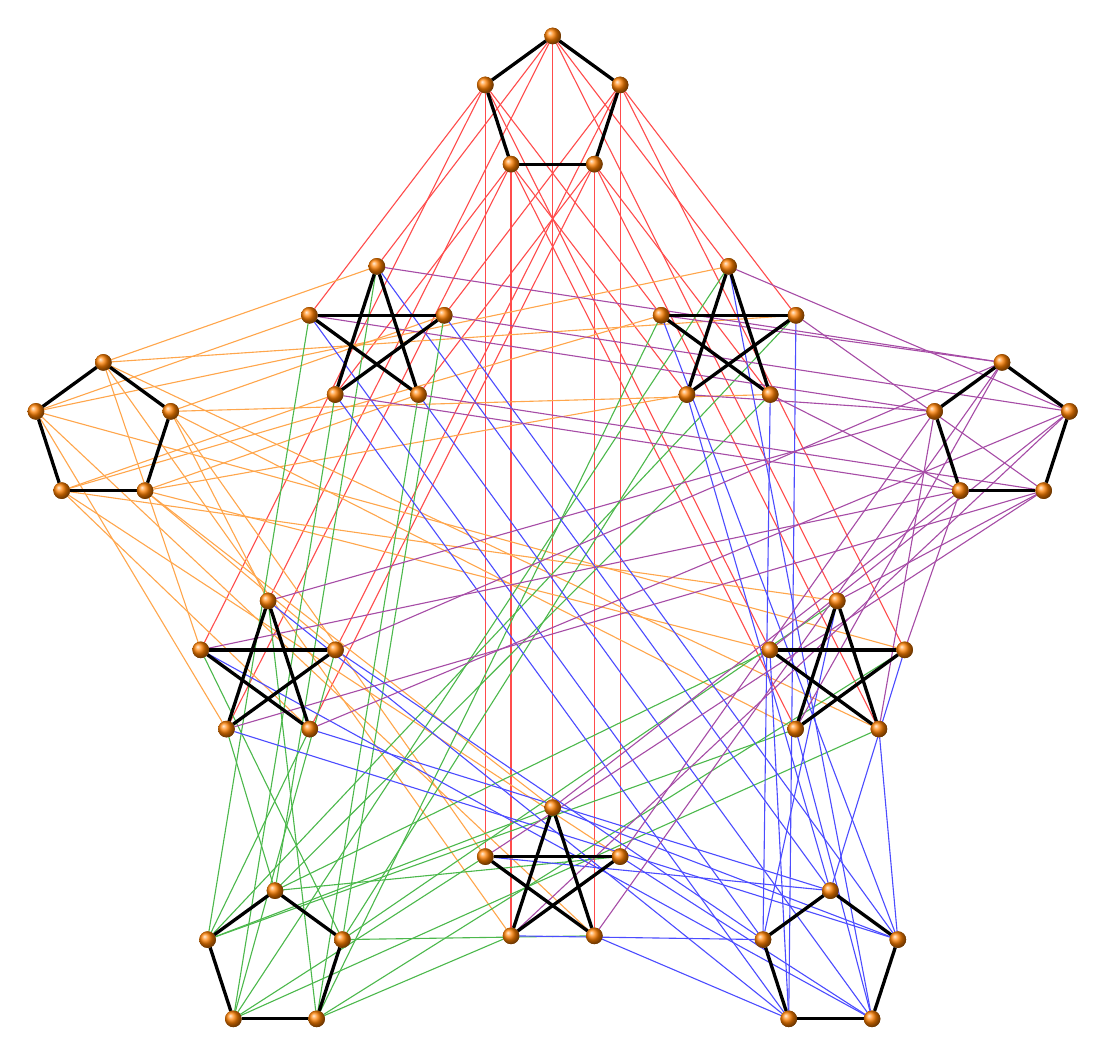
\begin{tikzpicture}
  \GraphInit[vstyle=Art]
  \SetVertexNoLabel
  \tikzset{VertexStyle/.append style = {minimum size = 6pt}}
  \def\R{6}\def\r{.9}
  \foreach \h in {0,...,4}{\foreach \j in {0,...,4}{%
    \pgfmathsetmacro\x{\R*cos(72*\h+90)+\r*cos(72*\j+90)}
    \pgfmathsetmacro\y{\R*sin(72*\h+90)+\r*sin(72*\j+90)}
    \Vertex[x=\x,y=\y]{P\h\j}
    \pgfmathsetmacro\x{(\R-2.2)*cos(72*\h+126)+\r*cos(72*\j+90)}
    \pgfmathsetmacro\y{(\R-2.2)*sin(72*\h+126)+\r*sin(72*\j+90)}
    \Vertex[x=\x,y=\y]{Q\h\j}}}
  \foreach \h/\c in {0/red,1/orange,2/green!60!black,3/blue,4/violet}{%
    \foreach \i in {0,...,4}{\foreach \j in {0,...,4}{%
      \pgfmathtruncatemacro\k{mod(\h*\i+\j,5)}
      \Edge[local,color=\c!70,lw=.4pt](P\h\j)(Q\i\k)}}}
  \foreach \h in {0,...,4}{%
    \Edges[local,lw=1.2pt](P\h0,P\h1,P\h2,P\h3,P\h4,P\h0)
    \Edges[local,lw=1.2pt](Q\h0,Q\h2,Q\h4,Q\h1,Q\h3,Q\h0)}
  \foreach \h in {0,...,4}{\foreach \j in {0,...,4}{%
    \Vertex[Node]{P\h\j}\Vertex[Node]{Q\h\j}}}
\end{tikzpicture}
\end{document}
